%%%%%%%%%%%%%%%%%%%%%%%%%%%%%%%%%%%%%%%%%%%%%%%%%%%%%%%%%%%%%%%%%%%%%%
% LaTeX Template: Beamer arrows
%
% Source: http://www.texample.net/
% Feel free to distribute this template, but please keep the
% referal to TeXample.net.
% Date: Nov 2006
% 
%%%%%%%%%%%%%%%%%%%%%%%%%%%%%%%%%%%%%%%%%%%%%%%%%%%%%%%%%%%%%%%%%%%%%%
% How to use writeLaTeX: 
%
% You edit the source code here on the left, and the preview on the
% right shows you the result within a few seconds.
%
% Bookmark this page and share the URL with your co-authors. They can
% edit at the same time!
%
% You can upload figures, bibliographies, custom classes and
% styles using the files menu.
%
% If you're new to LaTeX, the wikibook is a great place to start:
% http://en.wikibooks.org/wiki/LaTeX
%
%%%%%%%%%%%%%%%%%%%%%%%%%%%%%%%%%%%%%%%%%%%%%%%%%%%%%%%%%%%%%%%%%%%%%%

\documentclass[usenames,dvipsnames]{beamer} %
\usetheme{Madrid}
\usecolortheme{beaver}
\usepackage[latin1]{inputenc}
\usefonttheme{professionalfonts}
\usepackage{pifont}
\usepackage{tikz}
\usepackage{amsmath,amsfonts,amssymb}
\usepackage{verbatim}
\usepackage{hyperref}
\usepackage{subfigure}

\usepackage{xcolor}
\usepackage{media9}
\usepackage{animate}
\usepackage{booktabs}
\usepackage{simpsons}
\usepackage{color}
\usepackage{listings}

\definecolor{deepblue}{rgb}{0,0,0.5}
\definecolor{deepred}{rgb}{0.6,0,0}
\definecolor{deepgreen}{rgb}{0,0.5,0}

\DeclareMathOperator*{\argmax}{arg\,max}
\DeclareMathOperator*{\argmin}{arg\,min}

\usetikzlibrary{arrows,shapes}

\beamerdefaultoverlayspecification{<+->}

\setbeamercolor{itemize item}{fg=red}
\setbeamercolor{itemize subitem}{fg=BrickRed}
\setbeamercolor{itemize subsubitem}{fg=black}

\setbeamertemplate{itemize item}[square]
\setbeamertemplate{itemize subitem}[circle]
\setbeamertemplate{itemize subsubitem}[triangle]

\setbeamertemplate{caption}[numbered]

\newcommand\bred[1]{\textcolor{red}{\textit{#1}}}
\newcommand\bblue[1]{\textcolor{blue}{\textit{#1}}}

\newcommand\vari[1]{\textcolor{BrickRed}{\texttt{#1}}}
\newcommand\defi[1]{\textcolor{NavyBlue}{\textit{#1}}}


\renewcommand{\figurename}{Figura}
\newcommand{\matr}[1]{\mathbf{#1}}

\author{MSc. Diego Porres}
\title{Elements of Machine Learning}
\subtitle{Regresi\'on Lineal}
\institute[UFM]{
\includegraphics[height=0.73cm, width=3.3cm]{images/LogotipoUFM_interna.png}}
\date{Enero 2019}


\begin{document}

\frame{\titlepage}

\begin{comment}
:Title: Beamer arrows
:Tags: Remember picture, Beamer, Physics & chemistry, Overlays
:Use page: 3

With PGF/TikZ version 1.09 and later, it is possible to draw paths between nodes across
different pictures. This is a useful feature for presentations with the
Beamer package. In this example I've combined the new PGF/TikZ's overlay feature
with Beamer overlays. Download the PDF version to see the result.

**Note.** This only works with PDFTeX, and you have to run PDFTeX twice.

| Author: Kjell Magne Fauske

\end{comment}


% For every picture that defines or uses external nodes, you'll have to
% apply the 'remember picture' style. To avoid some typing, we'll apply
% the style to all pictures.
\tikzstyle{every picture}+=[remember picture]

% By default all math in TikZ nodes are set in inline mode. Change this to
% displaystyle so that we don't get small fractions.
\everymath{\displaystyle}

\begin{frame}
\begin{center}
	Some of the figures in this presentation are taken from \textit{An Introduction to Statistical Learning, with applications in R}  (Springer, 2013) with permission from the authors: G. James, D. Witten,  T. Hastie and R. Tibshirani
\end{center}
\end{frame}

\begin{frame}\frametitle{Intro (1)}
    \begin{itemize}
        \item Queremos empezar a realizar aproximaciones de $f$ de manera m\'as formal.
        \item En el aprendizaje supervisado, empezaremos por el modelo de \textbf{regresi\'on lineal}.
        \item Generalmente, $f(x)=\mathbb{E}[y\arrowvert x]$ (la funci\'on de regresi\'on real) \textit{rara vez} es lineal.
        \item Sin embargo, nos sirve como un buen paso para desarrollar otros modelos, adem\'as de que es simple y f\'acil de interpretar.
    \end{itemize}
\end{frame}

\begin{frame}{Intro (2)}
	\begin{itemize}
		\item Regresi\'on \textit{lineal} debido a que $\hat{f}$ es lineal con respecto a los coeficientes.
		\item \textbf{Ventajas:}
		\begin{itemize}
			\item Puede superar a m\'etodos no lineales cuando uno tiene pocos ejemplos de entrenamiento y/o datos escasos.
			\item Podemos hacerlo \textit{no lineal} al aplicar transformaciones no lineales a los datos (e.g., elevalrlos al cuadrado, multiplicarlos, etc.).
		\end{itemize}
	\end{itemize}
\end{frame}

\begin{frame}{Intro (3)}
	\begin{itemize}
		\item En la motivaci\'on de la clase pasada, usamos los datos de \vari{Advertising}
		\[ \vari{ventas} \Longleftrightarrow \vari{TV}, \vari{radio}, \vari{peri\'odico}\]
		\item Nos interesa determinar:
		\begin{itemize}
			\item ?`Existe una relaci\'on entre las \vari{ventas} y los presupuestos para los distintos medios?
			\item Si la hay, ?`qu\'e tan fuerte es esa relaci\'on?
			\item ?`Cu\'al de los medios contribuye (m\'as) a las ventas?
			\item ?`Con qu� precisi\'on podemos predecir las ventas a futuro?
			\item ?`La relaci\'on es lineal?
			\item ?`Hay sinergia entre los medios publicitarios?
		\end{itemize}
	\end{itemize}
\end{frame}

\begin{frame}\frametitle{Datos de \vari{Advertising}}
    \begin{figure}
    \centering
        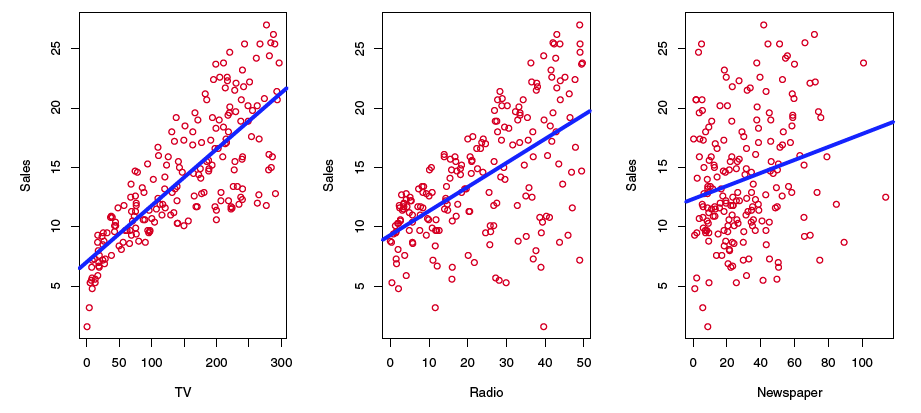
\includegraphics[width=0.70\textwidth]{images/islr/fig_2_1.png}
    \caption{Graficamos los datos de \vari{Advertising}. Los presupuestos de 200 mercados para la \vari{TV}, \vari{radio} y \vari{peri\'odico} est\'an en miles de d\'olares. La l\'inea azul representa la l\'inea de ajuste de m\'inimos cuadrados utilizando las variables respectivas.}
    \label{fig:2_advertising}
    \end{figure}
\end{frame}

\begin{frame}\frametitle{Regresi\'on Lineal con un predictor $X$}
	\begin{itemize}
		\item Asumimos que el modelo real de los datos es de la forma:
		\begin{equation}\label{eq:islr_3-1} 
		Y = \beta_0 + \beta_1 X + \epsilon \end{equation}
		donde $\beta_0$ y $\beta_1$ son dos constates desconocidas que representan el \defi{intercepto} y \defi{pendiente}, respectivamente, y $\epsilon$ es un t\'ermino de error.
		\item Llamamos tambi\'en a $\beta_0$ y a $\beta_1$ \defi{coeficientes} o \defi{par\'ametros}.
		\item Si tenemos estimados de los coeficientes del modelo, $\hat{\beta}_0$ y $\hat{\beta}_1$, entonces podemos predecir ventas futuras por medio de:
		\begin{equation}\label{eq:islr_3-2}
		\hat{y} = \hat f (x) = \hat{\beta}_0 + \hat{\beta}_1 x
		\end{equation}
		donde $\hat{y}$ indica una predicci\'on de $Y$ bas\'andonos en $X=x$.
	\end{itemize}
\end{frame}

\begin{frame}\frametitle{Estimando los Coeficientes}
	\begin{itemize}
		\item En otras palabras, usando el presupuesto de \vari{TV}, asumimos que la relaci\'on es lineal:
		\[ \vari{ventas} \approx \beta_0 + \beta_1 \times \vari{TV} \]
		
		\item Claramente, no sabemos los valores actuales de $\beta_0$ y $\beta_1$, por lo que debemos de usar a los datos para estimarlos.
		\item Obtendremos los coeficientes $\hat{\beta}_0$ y $\hat{\beta}_1$ usando a nuestros $n$ datos de entrenamiento $\mathcal{T}_{\text{Tr}}=\{(x_1,y_1),\dots,(x_n,y_n)\}$, con $x_i \in \mathbb{R}^p$ y $y_i \in \mathbb{R}$.
		\item Queremos que la l\'inea obtenida (i.e, los coeficientes obtenidos) est\'e lo m\'as \textbf{cerca} posible a los datos de entrenamiento.
	\end{itemize}
\end{frame}

\begin{frame}\frametitle{Criterio de M\'inimos Cuadrados}
\begin{itemize}
	\item Sea $\hat{y}_i = \hat{\beta}_0 + \hat{\beta}_1x_i$ la predicci\'on de $Y$ basados en el $i-$\'esimo valor de $X$.
	\item Definimos al $i-$\'esimo \defi{residual} como $e_i = y_i - \hat y_i$.
	\item Definimos a la \defi{suma residual de cuadrados (RSS)} como:
	
	\begin{equation}\label{eq:islr_3-3}
		\begin{aligned}
			\text{RSS}(\hat \beta) &= e_{1}^2 + \dots + e_{n}^2 \\
			&= (y_1 - \hat{\beta}_0 + \hat{\beta}_1x_1)^2 + \dots + (y_n - \hat{\beta}_0 + \hat{\beta}_1x_n)^2\\
			&= \sum_{i=1}^{n}(y_i - \hat{\beta}_0 + \hat{\beta}_1x_i)^2
		\end{aligned}
	\end{equation}
	\item El \defi{criterio de m\'inimos cuadrados} escoge a $\hat \beta_0$ y a $\hat \beta_1$ que minimizan a RSS $\Longleftrightarrow \hat \beta_0, \hat \beta_1 = \argmin_{\beta_0, \beta_1} \text{RSS}( \beta)$.
\end{itemize}
\end{frame}

\begin{frame}\frametitle{Soluci\'on a RSS}
	\begin{itemize}
		\item Usando c\'alculo, podemos encontrar que los valores de los coeficientes que minimizan a RSS son:
		\begin{equation}\label{eq:islr_3-4}
		\hat \beta_1 = \frac{\sum_{i=1}^{n}(x_i - \overline{x})(y_i - \overline{y})}{\sum_{i=1}^{n}(x_i - \overline{x})^2} \qquad \hat \beta_0 = \overline{y} - \hat \beta_1 \overline{x}
		\end{equation}
		donde $\overline{x} = \frac{1}{n}\sum_{i=1}^{n}x_i$ y $\overline{y} = \frac{1}{n}\sum_{i=1}^{n}y_i$.
		\item \'Estos coeficientes caracterizar\'an a la \defi{l\'inea de m\'inimos cuadrados}.
		\item Consiga a $\hat \beta_0$ y a $\hat \beta_1$ para los datos de \vari{Advertising}, con $X=\vari{TV}$ y $Y=\vari{sales}$.
	\end{itemize}
\end{frame}

\begin{frame}[fragile]\frametitle{C\'odigo RSS (1)}
\begin{semiverbatim}
	\small{\textcolor{deepblue}{import} numpy \textcolor{deepblue}{as} np
	\textcolor{deepblue}{import} pandas \textcolor{deepblue}{as} pd
	
	df = pd.read\_csv("Advertising.csv", index\_col=0)
	
	tv, ventas = df["TV"], df["sales"]
	
	tv\_prom = np.mean(tv)
	v\_prom = np.mean(ventas)
	
	b\_1 = np.sum((tv-tv\_prom)*(ventas-v\_prom)/np.sum((tv-tv\_prom)**2)\footnotemark \footnotetext{V\'ease \href{https://goo.gl/BdwXx3}{https://goo.gl/BdwXx3}.}
	b\_0 = v\_prom - b\_1*tv\_prom

	>>> b\_0
	7.0325935491276965
	>>> b\_1
	0.047536640433019736}
\end{semiverbatim}
\end{frame}
\text{ si la persona } i \text{ es estudiante}
\begin{frame}\frametitle{\vari{TV} vs. \vari{ventas}}
\begin{figure}
	\centering
	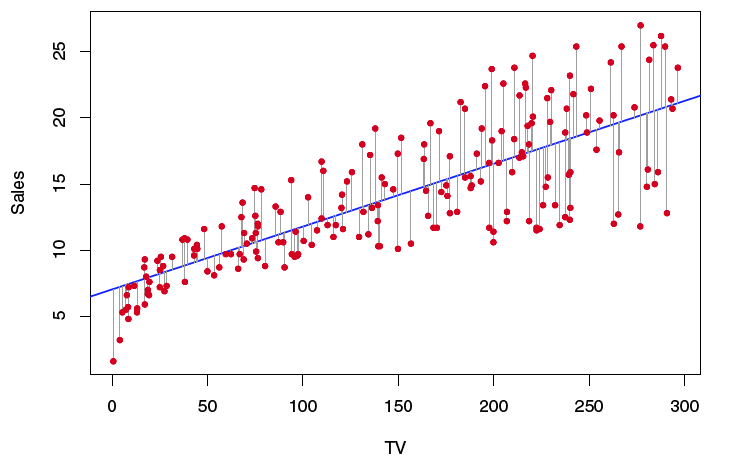
\includegraphics[width=0.7\textwidth]{images/islr/fig_3_1.png}
	\caption{Mostramos la l\'inea que minimiza RSS para los datos de \vari{Advertising}. N\'otese que es algo deficiente en la parte izquierda de la gr\'afica. $\hat \beta_0 = 7.03$ ser\'a el intercepto, mientras que $\hat \beta_1 = 0.0475$ ser\'a la pendiente, implicando que $\$1000$ m\'as invertidos en publicidad en \vari{TV} incrementar\'an las ventas en aproximadamente $47.5$ unidades.}
	\label{fig:1_3curvas_3}
\end{figure}
\end{frame}

\begin{frame}\frametitle{RSS en forma matricial}
\begin{itemize}
	\item Como hemos visto anteriormente, si tomamos a $y = (y_1, \dots, y_n)^{\top}$ y
	
	\[\beta = (\beta_0, \beta_1, \dots, \beta_p)^{\top} \qquad \matr{X} = \begin{pmatrix} 
	1 & x_{11} & x_{12} & \dots & x_{1p} \\
	1 & x_{21} & x_{22} & \dots & x_{2p} \\
	\vdots & \vdots & \vdots & \ddots & \vdots\\
	1 & x_{n1} & x_{n2} & \dots & x_{np}
	\end{pmatrix} \]
	tendremos en notaci\'on matricial:
	
	\begin{equation}\label{eq:esl_3-3}
	\text{RSS}(\beta) = (\matr{y} - \matr{X}\beta)^\top (\matr{y} - \matr{X}\beta)
	\end{equation}
	\item La soluci\'on, usando a la \textbf{ecuaci\'on normal}, es:
	
	\begin{equation}\label{eq:esl_3-6}
	\hat \beta = (\matr X^\top \matr X)^{-1} \matr{X}^\top \matr y
	\end{equation}
\end{itemize}
\end{frame}

\begin{frame}[fragile]\frametitle{C\'odigo RSS (2)}
\begin{semiverbatim}
	\small{\textcolor{deepblue}{import} numpy \textcolor{deepblue}{as} np
		\textcolor{deepblue}{import} pandas \textcolor{deepblue}{as} pd
		
		df = \href{https://pandas.pydata.org/pandas-docs/stable/generated/pandas.read_csv.html}{pd.read\_csv}("Advertising.csv", index\_col=0)
		
		tv, ventas = df["TV"], df["sales"]
		
		x = np.array(tv)
		y = np.array(ventas)
		
		X = \href{https://docs.scipy.org/doc/numpy-1.15.0/reference/generated/numpy.vstack.html}{np.vstack}([np.ones(len(x)), x]).T
		
		b\_0, b\_1 = np.linalg.inv(X.T.dot(X)).dot(X.T.dot(y))
		
		>>> b\_0
		7.032593549127698
		>>> b\_1
		0.047536640433019736}
\end{semiverbatim}
\end{frame}


\begin{frame}[fragile]\frametitle{C\'odigo RSS (3)}
\begin{semiverbatim}
	\small{\textcolor{deepblue}{import} numpy \textcolor{deepblue}{as} np
		\textcolor{deepblue}{import} pandas \textcolor{deepblue}{as} pd
		
		df = \href{https://pandas.pydata.org/pandas-docs/stable/generated/pandas.read_csv.html}{pd.read\_csv}("Advertising.csv", index\_col=0)
		
		tv, ventas = df["TV"], df["sales"]
		
		x = np.array(tv)
		y = np.array(ventas)
		
		X = \href{https://docs.scipy.org/doc/numpy-1.15.0/reference/generated/numpy.vstack.html}{np.vstack}([np.ones(len(x)), x]).T
		
		b\_0, b\_1 = np.linalg.lstsq(X, y)[0]
	
		rss = np.linalg.lstsq(X, y)[1]
>>> b\_1
	0.047536640433019736}
	
\end{semiverbatim}
\end{frame}

\begin{frame}\frametitle{?`Qu\'e tan exactas son las estimaciones de los coeficientes?}

\begin{figure}
	\centering
	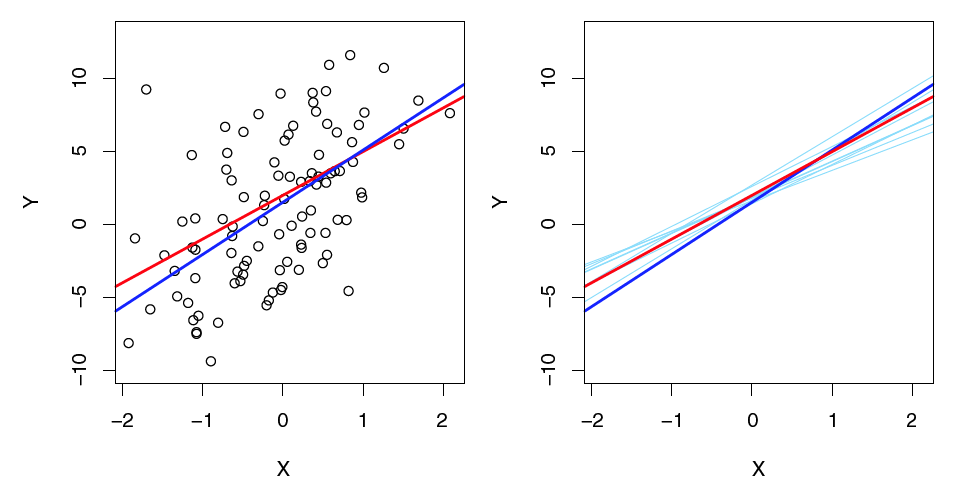
\includegraphics[width=0.7\textwidth]{images/islr/fig_3_3.png}
	\caption{A la izquierda se muestran en negro los datos simulados de la \defi{l\'inea de regresi\'on de la poblaci\'on} $Y=2+3X+\epsilon$ (en \textcolor{red}{rojo}) y la l\'inea de regresi\'on de m\'inimos cuadrados en \textcolor{blue}{azul}.  A la derecha mostramos las mismas l\'ineas, mas en \textcolor{Cerulean}{azul punteado} otras 10 l\'ineas de regresi\'on de m\'inimos cuadrados, tomando distintos conjuntos de entrenamiento.} 
	\label{fig:islr_3-3}
\end{figure}
\end{frame}

\begin{frame}\frametitle{Error Est\'andar Residual (RSS)}
	\begin{itemize}
		\item Podemos calcular el \defi{error est\'andar (SE)} de los coeficientes obtenidos para ver qu\'e tanto cambian bajo un muestreo repetido.
		\item Sea $\sigma^2 = \mathbb{V}(\epsilon)$:
		
		\begin{equation}\label{eq:islr_3-8-1}
		\text{SE}(\hat \beta_0)^2 = \sigma^2 \left[ \frac{1}{n} + \frac{\overline x^2}{\sum_{i=1}^{n}(x_i - \overline x)^2}\right]
		\end{equation}
		\begin{equation}\label{eq:islr_3-8-2}
		\text{SE}(\hat \beta_1)^2 = \frac{\sigma^2}{\sum_{i=1}^{n}(x_i - \overline x)^2}
		\end{equation}
		\item En general, no sabemos el valor de $\sigma^2$, por lo que lo estimamos de los datos y lo llamamos el \defi{error est\'andar residual (RSE)}:
		\begin{equation}
			\text{RSE} = \sqrt{\text{RSS}/(n-p-1)} = \sqrt{\text{RSS}/(n-2)}
		\end{equation}
	\end{itemize}
\end{frame}

\begin{frame}\frametitle{Intervalos de Confianza}
	\begin{itemize}
		\item Con los errores est\'andar, podemos calcular los \defi{intervalos de confianza (CI)} para cada coeficiente.
		\item El \defi{intervalo de confianza del 95\%} para $ \beta_0$ tiene la forma:
		
		\begin{equation}\label{eq:islr_3-11}
		\hat \beta_0 \pm 2\cdot \text{SE}(\hat \beta_0)
		\end{equation}
		
		y de igual manera para el CI de $ \beta_1$:
		
		\begin{equation}\label{eq:islr_3-9}
		\hat \beta_1 \pm 2\cdot \text{SE}(\hat \beta_1)
		\end{equation}
		
		\item Para los datos de \vari{Advertising}, el CI del 95\% para $\beta_0$ es $[6.130, 7.935]$, mientras que el CI del 95\% para $\beta_1$ es $[0.042, 0.053]$.
		\begin{itemize}
			\item En otras palabras, si no hay publicidad en \vari{TV}, las ventas caer\'an, en promedio, entre 6130 y 7935 unidades.
		\end{itemize}
	\end{itemize}
\end{frame}

\begin{frame}\frametitle{Pruebas de Hip\'otesis (1)}
	\begin{itemize}
		\item Utilizando a los errores est\'andar, tambi\'en podemos realizar las \defi{pruebas de hip\'otesis} de los coeficientes.
		\item Para recapitular, probamos a la \defi{hip\'otesis nula} de
		
		\begin{center}
			$H_0:$ No hay relaci\'on entre $X$ y $Y$
		\end{center}
		versus la \defi{hip\'otesis alterna}
		\begin{center}
			$H_a:$ Hay alguna relaci\'on entre $X$ y $Y$
		\end{center}
		\item De forma matem\'atica, tendremos de forma equivalente:
		\begin{equation*}
			H_0:\beta_1=0 
		\end{equation*}
		versus
		\begin{equation*}
		H_a:\beta_1\neq0
		\end{equation*}
		lo cual implicar\'ia que $Y=\beta_0 + \epsilon$ y entonces $X$ no est\'a asociado a $Y$.
	\end{itemize}
\end{frame}

\begin{frame}\frametitle{Pruebas de Hip\'otesis (2)}
\tikzstyle{na} = [baseline=-.5ex]
	\begin{itemize}
		\item Para probar a la hip\'otesis nula, calculamos el \defi{valor t} dado por:
		
		\begin{equation}\label{eq:islr_3-14}
			t=\tikz[baseline]{
				\node[anchor=east] (t2)
				{$\frac{\hat \beta_1 - 0}{\text{SE}(\hat \beta_1)}$};}
		\end{equation}
		\begin{itemize}
			\item Ya que $H_0:\beta_1=0$ \tikz[na]\node [coordinate] (n2) {};
			\item Tendr\'a una distribuci\'on $t$ con $n-p-1=n-2$ grados de libertad.
		\end{itemize}
		\begin{tikzpicture}[overlay]
		\path[->]<2-> (n2) edge [out=-10, in=25, looseness=2.3] (t2);
		\end{tikzpicture}
		\item Podremos calcular la probabilidad de observar cualquier valor igual o mayor a $\lvert t\rvert$ asumiendo que la hip\'otesis nula es cierta: el \defi{valor p}.
		\item Si el valor p es muy bajo (menor a e.g. 5 o 1\%), podemos rechazar a la hip\'otesis nula.
	\end{itemize}
\end{frame}

\begin{frame}[fragile]\frametitle{C\'odigo prueba de hip\'otesis}
\begin{semiverbatim}
	\small{\textcolor{deepblue}{import} statsmodels.formula.api \textcolor{deepblue}{as} smf
		\textcolor{deepblue}{import} pandas \textcolor{deepblue}{as} pd
		
		df = \href{https://pandas.pydata.org/pandas-docs/stable/generated/pandas.read_csv.html}{pd.read\_csv}("Advertising.csv", index\_col=0)
		
		est = smf.ols(formula="sales ~ TV", data=df).fit()
		
		>>> print(est.summary().tables[1])
		
		==============================================================
		              coef  std err        t   P>|t|   [0.025   0.975]
		--------------------------------------------------------------
		Intercept   7.0326    0.458   15.360   0.000    6.130    7.935
		TV          0.0475    0.003   17.668   0.000    0.042    0.053
		==============================================================}
\end{semiverbatim}
\end{frame}

\begin{frame}\frametitle{?`Qu\'e tan exacto es el modelo? - RSE}
	\begin{itemize}
		\item Media vez hemos rechazado a la hip\'otesis nula, debemos de cuantificar la medida en que el modelo se ajusta a los datos.
		\item El \defi{error est\'andar residual (RSE)} es una estimaci\'on de la desviaci\'on est\'andar de $\epsilon$ (i.e., la cantidad promedio que la variable de salida se desviar\'a de la verdadera l\'inea de regresi\'on):
		
		\begin{equation}\label{eq:islr_3-15}
		\text{RSE} = \sqrt{\frac{1}{n-2}\text{RSS}} = \sqrt{\frac{1}{n-2}\sum_{i=1}^{n}(y_i-\hat y_i)^2}
		\end{equation}
		\item Con el modelo pasado, lo conseguimos de la siguiente manera\footnotemark \footnotetext{V\'ease \href{https://goo.gl/nnJyxf}{https://goo.gl/nnJyxf}.}: \texttt{est.scale**0.5=3.258656}.
		\item \'Esto implica que, aunque el modelo fuese correcto y tuvi\'esemos los valores exactos de $\beta_0$ y $\beta_1$, cualquier predicci\'on de las \vari{venta} en base a la publicidad en la \vari{TV} estar\'ia equivocado en casi 3260 unidades en promedio.
	\end{itemize}
\end{frame}

\begin{frame}\frametitle{?`Qu\'e tan exacto es el modelo? - $R^2$}
\begin{itemize}
	\item No siempre se tiene claro qu\'e constituye un buen RSE.
	\item EL estad\'istico \defi{$R^2$} es la fracci\'on o proporci\'on de la varianza de $Y$ explicada usando a $X$, i.e.:
	
	\begin{equation}\label{eq:islr_3-17}
	R^2=\frac{\text{TSS}-\text{RSS}}{\text{TSS}}=1-\frac{\text{RSS}}{\text{TSS}}
	\end{equation}
	donde $\text{TSS}=\sum_{i=1}^{n}(y_i - \overline{y})^2$ es la \defi{suma total de cuadrados}.
	\item En F\'isica, $R^2\approx1$ puede ser f\'acilmente obtenido, mientras que en Biolog\'ia, Psicolog\'ia, Mercadeo, etc., $R^2<0.1$ es m\'as realista.
	\item \texttt{est.rsquared=0.611875}
\end{itemize}

\end{frame}

\begin{frame}\frametitle{?`Qu\'e tan exacto es el modelo? - $r$}
	\begin{itemize}
		\item Finalmente, podemos calcular otra medici\'on de la relaci\'on lineal entre $X$ y $Y$, su \defi{correlaci\'on}:
		\begin{equation}\label{eq:islr_3-18}
		\text{Cor}(X,Y)=\frac{\sum_{i=1}^{n}(x_i-\overline{x})(y_i - \overline{y})}{\sqrt{\sum_{i=1}^{n}(x_i-\overline{x})^2}\sqrt{\sum_{i=1}^{n}(y_i- \overline{y})^2}}
		\end{equation}
		\item Otra forma de escribirlo es $r=\text{Cor}(X,Y)$.
		\item Se puede demostrar que $r^2=R^2$.
		\item \texttt{np.corrcoef(df["TV"], df["sales"])[0][1]=0.78222442}
		\item \texttt{pearsonr(df["TV"], df["sales"])[0]=0.78222442}
		\item Sin embargo, debido a que es una cantidad \textit{por pares}, no se extiende naturalmente a una regresi\'on m\'ultiple, mientras que el $R^2$ s\'i lo hace.
	\end{itemize}
\end{frame}

\begin{frame}\frametitle{Regresi\'on Lineal M\'ultiple}
	\begin{itemize}
		\item No podemos correr $p$ distintas regresiones lineales: ?`qu\'e pasa si los medios de publicidad est\'an correlacionados?
		\item Lo mejor es extender al modelo para que acomode multiples predictores (\defi{regresi\'on lineal m\'ultiple}):
		\begin{equation}\label{eq:islr_3-19}
			Y = \beta_0 + \beta_1 X_1 + \dots + \beta_p X_p + \epsilon
		\end{equation}
		\item Interpretamos a cada $\beta_j$ como el efecto \textit{promedio} sobre $Y$ si se incrementa a $X_j$ en una unidad, \textbf{fijando a todas las otras variables predictoras}.
		\item Para los datos de \vari{Advertising}, tendremos que el modelo se vuelve:
		
		\[ \vari{ventas} = \beta_0 + \beta_1 \times \vari{TV} + \beta_2 \times \vari{radio} + \beta_3 \times \vari{peri\'odico} + \epsilon \]
		\begin{itemize}
			\item \textit{"Essentially, all models are wrong, but some are useful" -George Box}
		\end{itemize}
	\end{itemize}
\end{frame}

\begin{frame}\frametitle{Estimando los Coeficientes de Regresi\'on M\'ultiple}
	\begin{itemize}
		\item Dadas las estimaciones $\hat \beta_0, \hat \beta_1, \dots, \hat \beta_p$, podemos hacer predicciones usando la ecuaci\'on:
		
		\begin{equation}\label{eq:islr_3-21}
		\hat y = \hat \beta_0 + \hat \beta_1 x_1 + \dots + \hat \beta_p x_p
		\end{equation}
		\item Estimamos a los coeficientes $ \beta_0, \beta_1, \dots, \beta_p$ como los valores que minimizan al RSS:
		
		\begin{equation}\label{eq:islr_3-22}
		\begin{aligned}
		\text{RSS}(\hat \beta)&= \sum_{i=1}^{n}(y_i-\hat y_i)^2\\
		&= \sum_{i=1}^{n}(y_i-\hat \beta_0 - \hat \beta_1 x_{i1} - \dotsb - \hat \beta_p x_{ip})^2
		\end{aligned}
		\end{equation}
		\item Se pueden encontrar f\'acilmente usando \texttt{Python} o \texttt{R}.
	\end{itemize}
\end{frame}


\begin{frame}\frametitle{Regresi\'on M\'ultiple para $p=2$}
\begin{figure}
	\centering
	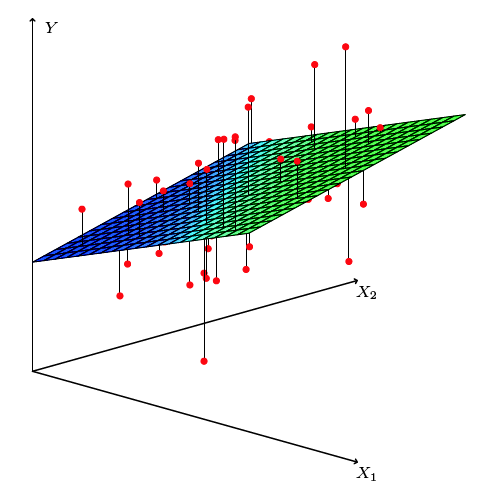
\includegraphics[width=0.45\textwidth]{images/islr/fig_3_4.png}
	\caption{Cuando $p=2$, tendremos datos en tres dimensiones, con dos predictores $X_1$ y $X_2$ y una variable de respuesta $Y$. En otras palabras, nuestra l\'inea de regresi\'on se convierte en un plano. Dicho plano se selecciona tal que se minimizen las distancias \textit{verticales} entre cada punto (en \textcolor{red}{rojo}) y el plano.}
	\label{fig:islr_3-4}
\end{figure}
\end{frame}

\begin{frame}[fragile]\frametitle{Coeficientes para Regresi\'on M\'ultiple}
\begin{semiverbatim}
	\footnotesize{\textcolor{deepblue}{import} statsmodels.formula.api \textcolor{deepblue}{as} smf
		\textcolor{deepblue}{import} pandas \textcolor{deepblue}{as} pd
		
		df = \href{https://pandas.pydata.org/pandas-docs/stable/generated/pandas.read_csv.html}{pd.read\_csv}("Advertising.csv", index\_col=0)
		
		est = smf.ols(formula="sales ~ TV+radio+newspaper", data=df).fit()
		
		>>> print(est.summary().tables[1])
		
		========================================================================
		                 coef    std err          t     P>|t|    [0.025   0.975]
		------------------------------------------------------------------------
		Intercept      2.9389      0.312      9.422     0.000     2.324    3.554
		TV             0.0458      0.001     32.809     0.000     0.043    0.049
		radio          0.1885      0.009     21.893     0.000     0.172    0.206
		newspaper     -0.0010      0.006     -0.177     0.860    -0.013    0.011
		========================================================================
	}
\end{semiverbatim}
\end{frame}

\begin{frame}\frametitle{An\'alisis}
\begin{itemize}
	\item Vemos que el valor p de \vari{peri\'odico} no es significativo.
	\begin{itemize}
		\item ?`Por qu\'e?
	\end{itemize}
	\item La diferencia entre las regresiones lineales simples y m\'ultiples es que en la primera se obtienen los coeficientes ignorando a todas las otras variables predictoras, mientras que en la \'ultima se toman a las otras variables como \textit{fijas}.
	\item Podemos obtener la matriz de correlaci\'on completa $\text{Cor}(X,Y)$ de la siguiente manera:  \texttt{df.corr()}
\end{itemize}
\end{frame}

\begin{frame}[fragile]\frametitle{Matriz de Correlaci\'on $\text{Cor}(X, Y)$}
\begin{semiverbatim}
		\textcolor{deepblue}{import} pandas \textcolor{deepblue}{as} pd
		
		df = \href{https://pandas.pydata.org/pandas-docs/stable/generated/pandas.read_csv.html}{pd.read\_csv}("Advertising.csv", index\_col=0)
		
		>>> df.corr()
		
		               TV   radio  newspaper   sales
		TV        1.00000 0.05481    0.05665 0.78222
		radio     0.05481 1.00000    0.35410 0.57622
		newspaper 0.05665 0.35410    1.00000 0.22830
		sales     0.78222 0.57622    0.22830 1.00000
\end{semiverbatim}
\end{frame}

\begin{frame}\frametitle{\vari{radio} vs. \vari{ventas}}
	\begin{itemize}
		\item Si el modelo de regresi\'on m\'ultiple es correcto, entonces el presupuesto invertido en \vari{radio} est\'a relacionado a las ventas, mientras que el invertido en \vari{peri\'odico} no.
		\item Analizando a la matriz de correlaci\'on, vemos que \vari{radio} y \vari{peri\'odico} tienen una correlaci\'on de $0.35410$.
		\item Es decir, se gasta m\'as en \vari{peri\'odico} en mercados donde se invierte m\'as en \vari{radio}.
		\item Por lo tanto, si hacemos una regresi\'on lineal simple de $\vari{ventas}\sim\vari{peri\'odico}$, obtendremos que s\'i existe relaci\'on, mas solamente es reflejo del efecto de \vari{radio} en dichos mercados.
	\end{itemize}
\end{frame}

\begin{frame}\frametitle{Algunas preguntas importantes...}
	\begin{itemize}
		\item Cuando realizamos regresi\'on lineal m\'ultiple sobre un conjunto de datos, usualmente nos interesa responder las siguientes preguntas:
		\begin{itemize}
			\item[1.] ?`Al menos uno de los predictores $X_1,\dots,X_p$ es \'util para predecir a la respuesta $Y$?
			\item[2.] ?`Todos los predictores ayudan a explicar a $Y$ o solo es \'util un subconjunto de ellos?
			\item[3.] ?`Qu\'e tan bien se ajusta el modelo a los datos?
			\item[4.] Dado un conjunto de predictores, ?`qu\'e valor de respuestas $Y$ deber\'iamos de predecir y cu\'an precisa es nuestra predicci\'on?
		\end{itemize}
	\end{itemize}
\end{frame}

\begin{frame}\frametitle{1. ?`Al menos uno de los predictores $X_1,\dots,X_p$ es \'util para predecir a la respuesta $Y$?}

\begin{itemize}
	\item Tendremos una prueba de hip\'otesis:
	
	\begin{equation*}
	H_0:\beta_1=\beta_2=\dotsb=\beta_p=0 
	\end{equation*}
	versus
	\begin{equation*}
	H_a:\text{ al menos un }\beta_j \text{ no es cero} 
	\end{equation*}
	\item Realizamos esta prueba de hip\'otesis utilizando el \defi{estad\'istico F}:
	\begin{equation}\label{eq:islr_3-23}
	F=\frac{(TSS-RSS)/p}{RSS/(n-p-1)}\sim F_{p,n-p-1}
	\end{equation}
	\item Si $H_0$ es correcto, $F\approx1$, mientras que si $H_a$ es correcto, $F>1$.
	\begin{itemize}
		\item Si $n$ es grande, $F>1$ para rechazar a $H_0$.
		\item Si $n$ es peque\~no, $F\gg 1$ para rechazar a $H_0$.
		\item Si $p>n$, no podemos siquiera calcular a la recta de m\'inimos cuadrados.
	\end{itemize}
\end{itemize}

\end{frame}

\begin{frame}[fragile]\frametitle{C\'odigo para el estad\'istico $F$}
\begin{semiverbatim}
	\footnotesize{>>> print(est.summary())
		                            OLS Regression Results                            
		========================================================================
		Dep. Variable:               sales   R-squared:                    0.897
		Model:                         OLS   Adj. R-squared:               0.896
		Method:              Least Squares   F-statistic:                  570.3
		Date:             lun, 14 ene 2019   Prob (F-statistic):        1.58e-96
		Time:                     16:10:44   Log-Likelihood:             -386.18
		No. Observations:              200   AIC:                          780.4
		Df Residuals:                  196   BIC:                          793.6
		Df Model:                        3                                         
		Covariance Type:         nonrobust                                         
		========================================================================
		                 coef    std err          t     P>|t|    [0.025   0.975]
		------------------------------------------------------------------------
		Intercept      2.9389      0.312      9.422     0.000     2.324    3.554
		TV             0.0458      0.001     32.809     0.000     0.043    0.049
		radio          0.1885      0.009     21.893     0.000     0.172    0.206
		newspaper     -0.0010      0.006     -0.177     0.860    -0.013    0.011
		========================================================================
	}
\end{semiverbatim}
\end{frame}

\begin{frame}\frametitle{2. ?`Todos los predictores ayudan a explicar a $Y$ o solo es \'util un subconjunto de ellos?}

\begin{itemize}
	\item Si rechazamos a $H_0$, ?`cu\'al de los predictores no nos sirve?
	\item Podemos realizar la regresi\'on con \defi{todos los subconjuntos} o \defi{mejor subconjunto} y seleccionar el "mejor" modelo.
	\begin{itemize}
		\item \textbf{Problema:} !`hay $\sum_{i=0}^{p}{p \choose i}=2^p$ subconjuntos/modelos!
		\item No hay mucho problema si $p$ es peque\~no, pero s\'i lo es para $p$ \textit{grandes}.
		\item Si $p=40$, hay $2^{40}\approx10^9$ distintos modelos a considerar.
	\end{itemize}
	\item Necesitamos formas automatizadas y eficientes para escoger un conjunto m\'as peque\~no de modelos a considerar. 
\end{itemize}

\end{frame}

\begin{frame}\frametitle{\defi{Forward selection}}
	\begin{itemize}
		\item Empezamos por el \defi{modelo nulo} ($\beta_j = 0, j\neq 0$).
		\item Ajustamos $p$ regresiones lineales simples y le agregamos al modelo nulo la variable que logra menor RSS.
		\item Agregamos a este modelo la variable que tenga menor RSS de todos los modelos con dos variables.
		\item Continuamos hasta llegar a una condici\'on de parada. 
		\item Siempre se puede usar.
		\item Puede incluir variables que m\'as adelante se vuelvan redundantes (e.g., incluir a \vari{peri\'odico} modelando a los datos de \vari{Advertising}).
		\end{itemize}
\end{frame}

\begin{frame}\frametitle{\defi{Backward selection}}
\begin{itemize}
	\item Empezamos con todas las variables del modelo y quitamos la que tiene el valor p m\'as grande.
	\item Ajustamos el modelo con $p-1$ variables y quitamos la variable con el valor p m\'as grande.
	\item Continuamos hata llegar a una condici\'on, e.g., a que todos los valores p est\'en por debajo de un l\'imite.
	\item No se puede usar si $p>n$.
\end{itemize}
\end{frame}

\begin{frame}\frametitle{\defi{Mixed selection}}
\begin{itemize}
	\item Combinaci\'on de forward y backward selection.
	\item Empezamos igual que en forward selection, solo que si en cualquier punto el valor p de las variables cruza cierto umbral, la quitamos del modelo.
	\item Continuamos hasta que todas las variables del modelo tengan un valor p lo suficientemente peque\~no \textbf{y} todas las variables fuera del modelo tienen un valor p grande si se agregan al modelo.
	\item Arregla el error de forward selection de incluir variables que luego se vuelven redundantes.
\end{itemize}
\end{frame}

\begin{frame}\frametitle{3. ?`Qu\'e tan bien se ajusta el modelo a los datos?}
	\begin{itemize}
		\item Vimos anteriormente que $R^2=0.8972$ cuando tenemos el modelo $\vari{ventas} \sim \vari{TV}+\vari{radio}+\vari{peri\'odico}$.
		\item Sin embargo, $R^2=0.89719$ si $\vari{ventas} \sim \vari{TV}+\vari{radio}$.
		\item $R^2$ siempre va a incrementar mientras m\'as variables incluyamos, aunque \'estas tengan un valor p muy alto.
		\item Es \'util realizar otras mediciones, como por ejemplo el RSE.
		\item Asimismo, es \'util inspeccionar  los datos de manera visual siempre que sea posible (o usando m\'etodos avanzados).
	\end{itemize}
\end{frame}

\begin{frame}\frametitle{Plano de regresi\'on para $\vari{ventas} \sim \vari{TV}+\vari{radio}$}
\begin{figure}
	\centering
	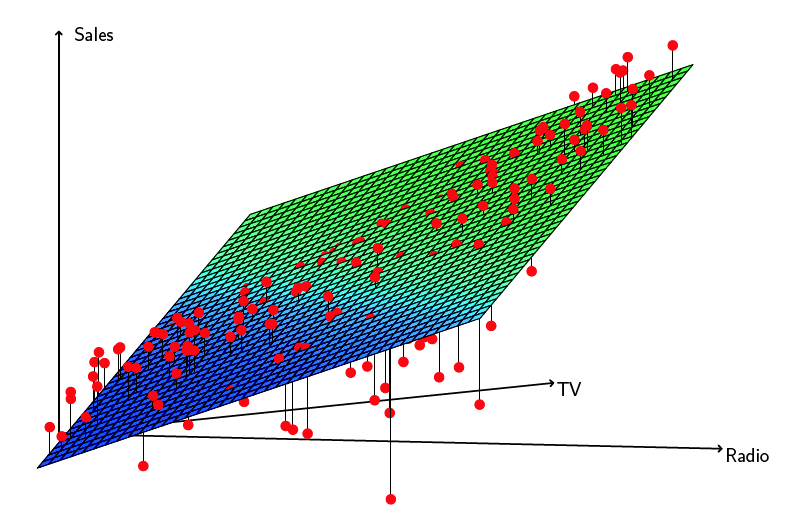
\includegraphics[width=0.6\textwidth]{images/islr/fig_3_5.png}
	\caption{Vemos la regresi\'on lineal ajustado a \vari{ventas} usando como predictores a \vari{TV} y a \vari{radio}. El modelo sobreestima a las \vari{ventas} cuando se gasta \'unicamente en \vari{TV} o en \vari{radio} y subestima cuando el presupuesto es dividido entre los dos medios. Sugiere una \textit{sinerg\'ia} entre los medios, donde una combinaci\'on de estos mejora las ventas m\'as que invirtiendo solamente en un medio.}
	\label{fig:islr_3-5}
\end{figure}
\end{frame}

\begin{frame}\frametitle{4. Dado un conjunto de predictores, ?`qu\'e valor de respuestas $Y$ deber\'iamos de predecir y cu\'an precisa es nuestra predicci\'on?}
	\begin{itemize}
		\item Teniendo a nuestro modelo, podemos predecir a la respuesta $Y$ con un dato nuevo $X$.
		\item Sin embargo, habr\'an tres fuentes de incertidumbre:
		\begin{itemize}
			\item La inexactitud en la estimaci\'on de los coeficientes est\'a relacionada al \textit{error reducible}.
			\item El \defi{sesgo del modelo}, i.e., que asumamos que el modelo sea lineal.
			\item El \textit{error irreducible} debido a $\epsilon$. Por lo tanto, podemos realizar \defi{intervalos de predicci\'on} (usualmente m\'as anchos que los CI) ya que incluyen al error reducible y al irreducible.
		\end{itemize}
	\end{itemize}
\end{frame}

\begin{frame}\frametitle{Predictores cualitativos (1)}
	\begin{itemize}
		\item Usualmmente algunos predictores son \defi{cualitativos} o \defi{categ\'oricos}, tomando solamente valores de un conjunto discreto.
		\item Para los datos de \vari{Credit}, tendremos 7 predictores cuantitativos y 4 cualitativos: \vari{Gender}, \vari{Student} (estado de estudiante), \vari{Married} (estado marital) y \vari{Ethnicity} (Cauc\'asico, Afroamericano o Asi\'atico).
	\end{itemize}
\end{frame}

\begin{frame}\frametitle{Los datos de \vari{Credit}}
\begin{figure}
	\centering
	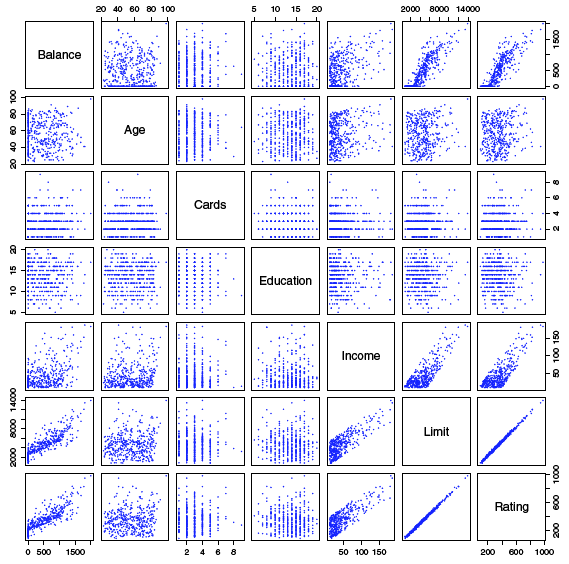
\includegraphics[width=0.54\textwidth]{images/islr/fig_3_6.png}
	\caption{\texttt{\textcolor{deepblue}{import} seaborn \textcolor{deepblue}{as} sns;}
			
			\href{https://seaborn.pydata.org/generated/seaborn.pairplot.html}{\texttt{sns.pairplot(credit)}}
	}
	\label{fig:islr_3-6}
\end{figure}
\end{frame}

\begin{frame}\frametitle{Predictores cualitativos (2)}
	\begin{itemize}
		\item Siguiendo analizando los datos de \vari{Credit}, queremos ver las diferencias entre hombres y mujeres.
		\item Por lo tanto, creamos una nueva \defi{variable ficticia} \defi{de dos niveles}:
		\begin{equation}\label{eq:islr_3-26}
			x_i = \begin{cases}
			0 & \text{ si la persona } i \text{ es mujer}\\
			1 & \text{ si la persona } i \text{ es hombre}
			\end{cases}
		\end{equation}
		\item Usando a esta variable, obtenemos el modelo $y_i = \beta_0 + \beta_1 x_i +\epsilon_i$ donde:
		\begin{equation}\label{eq:islr_3-27}
		y_i = \begin{cases}
		\beta_0+\epsilon_i & \text{ si la persona } i \text{ es mujer}\\
		\beta_0+\beta_1+\epsilon_i & \text{ si la persona } i \text{ es hombre}
		\end{cases}
		\end{equation}
		\begin{itemize}
			\item $\beta_0+ \beta_1$ es el balance en la tarjeta de cr\'edito promedio para los hombres 
			\item $\beta_0 $ el balance en la tarjeta de cr\'edito promedio para las mujeres
		\end{itemize}
	\end{itemize}
\end{frame}

\begin{frame}[fragile]\frametitle{\vari{Gender} vs. \vari{Balance}}
\begin{semiverbatim}
	\footnotesize{\textcolor{deepblue}{import} statsmodels.formula.api \textcolor{deepblue}{as} smf
		\textcolor{deepblue}{import} pandas \textcolor{deepblue}{as} pd
		
		credit = \href{https://pandas.pydata.org/pandas-docs/stable/generated/pandas.read_csv.html}{pd.read\_csv}("Credit.csv", usecols=list(range(1,12)))
		
		est = smf.ols(formula="Balance ~ Gender", data=credit).fit()
		
		>>> print(est.summary().tables[1])
		
		========================================================================
		                     coef  std err        t   P>|t|  [0.025      0.975]
		------------------------------------------------------------------------
		Intercept        529.5362  	31.988  	16.554  	0.000  	466.649	  592.423
		Gender[T.Male]   -19.7331  	46.051  	-0.429  	0.669  -110.267   	70.801
		========================================================================
	}
\end{semiverbatim}
\footnotetext{No es estad\'isticamente significativo.}
\end{frame}


\begin{frame}\frametitle{Predictores cualitativos (3)}
	\begin{itemize}
		\item Con mas de dos niveles, podemos crear variables ficticias adicionales.
		\item Por ejemplo, para la variable \vari{Ethnicity}, creamos dos variables ficticias:
		\begin{equation}\label{eq:islr_3-28}
		x_{i1} = \begin{cases}
		0 & \text{ si la persona } i \text{ es Asi\'atica}\\
		1 & \text{ si la persona } i \text{ no es Asi\'atica}
		\end{cases}
		\end{equation}
		y:
		\begin{equation}\label{eq:islr_3-29}
		x_{i2} = \begin{cases}
		0 & \text{ si la persona } i \text{ es Cauc\'asica}\\
		1 & \text{ si la persona } i \text{ no es Cauc\'asica}
		\end{cases}
		\end{equation}
		\item Como en el caso de dos niveles, la elecci\'on de dichas variables son totalmente aleatorias.
	\end{itemize}
\end{frame}

\begin{frame}\frametitle{Predictores cualitativos (4)}
	\begin{itemize}
		\item Tendremos como resultado el modelo $y_i = \beta_0 + \beta_1 x_{i1} +\beta_2 x_{i2} + \epsilon_i$ donde:
		\begin{equation}\label{eq:islr_3-30}
		y_i = \begin{cases}
		\beta_0+\beta_1+\epsilon_i & \text{ si la persona } i \text{ es Asi\'atica}\\
		\beta_0+\beta_2+\epsilon_i & \text{ si la persona } i \text{ es Cauc\'asica}\\
		\beta_0 + \epsilon_i & \text{ si la persona } i \text{ es Afroamericana}
		\end{cases}
		\end{equation}
		\begin{itemize}
			\item $\beta_0$ es el balance en la tarjeta de cr\'edito promedio para los Afroamericanos
			\item $\beta_1$ es la diferencia promedio en el balance de la tarjeta de cr\'edito entre Asi\'aticos y Afroamericanos 
			\item $\beta_2$ es la diferencia promedio en el balance de la tarjeta de cr\'edito entre Cauc\'asicos y Afroamericanos 
		\end{itemize}
	\item El nivel sin variable ficticia, Afroamericanos en este caso, se llama la \defi{base}.
	\end{itemize}
\end{frame}

\begin{frame}[fragile]\frametitle{\vari{Ethnicity} vs. \vari{Balance}}
\begin{semiverbatim}
	\footnotesize{\textcolor{deepblue}{import} statsmodels.formula.api \textcolor{deepblue}{as} smf
		\textcolor{deepblue}{import} pandas \textcolor{deepblue}{as} pd
		
		credit = \href{https://pandas.pydata.org/pandas-docs/stable/generated/pandas.read_csv.html}{pd.read\_csv}("Credit.csv", usecols=list(range(1,12)))
		
		est = smf.ols(formula="Balance ~ Ethnicity", data=credit).fit()
		
		>>> print(est.summary().tables[1])
		
		========================================================================
		                            coef std err      t  P>|t|  [0.025    0.975]
		------------------------------------------------------------------------
		Intercept                 531.00  46.319 11.464	 0.000   439.939  622.06
		Ethnicity[T.Asian]       -18.686  65.021	-0.287  0.774  -146.515  109.14
		Ethnicity[T.Caucasian]  -12.5025  56.681	-0.221  0.826  -123.935  98.930
		========================================================================
	}
\end{semiverbatim}
\end{frame}

\begin{frame}\frametitle{Extensiones al Modelo Lineal}
	\begin{itemize}
		\item Hemos estado asumiendo que la relaci\'on entre los predictores y la respuesta es \textit{aditiva} y \textit{linear}.
		\item La suposici\'on \defi{aditiva} quiere decir que el efecto de un cambio del predictor $X_j$ es independiente de los valores de los otros predictores.
		\item La suposici\'on \defi{lineal} quiere decir que el cambio en la respuesta $Y$ debido al incremento de $X_j$ por una unidad es constante, sin importar el valor de $X_j$.
		\item ?`Qu\'e sucede si relajamos estas dos suposiciones?
	\end{itemize}
\end{frame}


\begin{frame}\frametitle{Quitando la suposici\'on aditiva}
	\begin{itemize}
		\item Para los datos de \vari{Advertising}, las pendientes $\beta_1,\beta_2,\beta_3$ representan el efecto sobre las \vari{ventas} al incrementar en uno al presupuesto respectivo, sin importar cu\'anto se invirti\'o en los otros medios.
		\item Invertir en \vari{radio} usualmente incrementa la efectividad de la publicidad mostrada en \vari{TV}.
		\item Si tenemos un presupuesto de $\$100,000$, invertir la mitad en \vari{TV} y la mitad en \vari{radio} puede incrementar m\'as las ventas que invertirlo todo en \vari{TV} o en \vari{radio}.
		\item A \'esto se le conoce como un \defi{ efecto de sinergia} en mercadeo; en estad\'istica se conoce como un \defi{efecto de interacci\'
		on}.
	\begin{itemize}
		\item Lo vimos en la Figura \ref{fig:islr_3-5} con el modelo $\vari{ventas}\sim \vari{TV} + \vari{radio}$.
	\end{itemize}
	\end{itemize}
\end{frame}

\begin{frame}\frametitle{Modelando interacciones}
	\begin{itemize}
		\item Nuestro modelo tiene entonces la forma
		\begin{equation}\label{eq:islr_3-33}
		\begin{split}
		\vari{ventas} &= \beta_0 + \beta_1 \times \vari{TV} + \beta_2 \times \vari{radio} + \beta_3 \times (\vari{radio}\times\vari{TV}) + \epsilon\\
		&=\beta_0 + (\beta_1 + \beta_3 \times \vari{radio})\times \vari{TV} + \beta_2 \times \vari{radio}  + \epsilon\\
		&=\beta_0 + \widetilde{\beta}_1 \times \vari{TV} + \beta_2 \times \vari{radio} + \epsilon
		\end{split}
		\end{equation}
		con $\widetilde{\beta}_1=\beta_1+\beta_3\times\vari{radio}$, i.e., aumentar el presupuesto de \vari{radio} afectar\'a la efectividad de publicidad en \vari{TV}.
	\end{itemize}
\end{frame}

\begin{frame}[fragile]\frametitle{C\'odigo para interacciones}
\begin{semiverbatim}
	\footnotesize{est = smf.ols("sales~TV+radio+TV*radio, data).fit(); print(est.summary())
		                            OLS Regression Results                            
		==========================================================================
		Dep. Variable:                  sales   R-squared:                   0.968
		Model:                            OLS   Adj. R-squared:              0.967
		Method:                 Least Squares   F-statistic:                 1963.
		Date:                Wed, 16 Jan 2019   Prob (F-statistic):      6.68e-146
		Time:                        02:23:17   Log-Likelihood:            -270.14
		No. Observations:                 200   AIC:                         548.3
		Df Residuals:                     196   BIC:                         561.5
		Df Model:                           3                                         
		Covariance Type:            nonrobust                                         
		==========================================================================
		                coef    std err         t     P>|t|      [0.025     0.975]
		--------------------------------------------------------------------------
		Intercept     6.7502      0.248    27.233     0.000       6.261      7.239
		TV            0.0191      0.002    12.699     0.000       0.016      0.022
		radio         0.0289      0.009     3.241     0.001       0.011      0.046
		TV:radio      0.0011   5.24e-05    20.727     0.000       0.001      0.001
		==========================================================================
	}
\end{semiverbatim}
\end{frame}

\begin{frame}\frametitle{Interpretaci\'on}
	\begin{itemize}
		\item Vemos que el t\'ermino de interacci\'on es significativo, por lo que hay evidencia en contra de $H_0$.
		\item Ahora $R^2=0.968$, comparado con el modelo $\vari{ventas} \sim \vari{TV}+\vari{radio}$ donde obtuvimos $R^2=0.897$.
		\begin{itemize}
			\item \'Esto implica que el
			\[ \frac{0.968-0.897}{1-0.897}=0.689=68.9\% \]
			de la variabilidad en las \vari{ventas} que quedan despu\'es de ajustar el modelo $\vari{ventas} \sim \vari{TV}+\vari{radio}$ es explicado por el nuevo t\'ermino de interacci\'on $\vari{TV}\times\vari{radio}$.
			\item Por ende, un incremento en $\$1,000$ al presupuesto de \vari{TV} est\'a asociado a un incremento en las ventas de 
			\[ (\hat \beta_1 + \hat \beta_3 \times \vari{radio})\times1000=19.1 + 1.1\times\vari{radio}\text{ unidades}  \]
			\item Por ende, un incremento en $\$1,000$ al presupuesto de \vari{radio} est\'a asociado a un incremento en las ventas de 
			\[ (\hat \beta_2 + \hat \beta_3 \times \vari{TV})\times1000=28.9 + 1.1\times\vari{TV}\text{ unidades}  \]
		\end{itemize}
	\end{itemize}
\end{frame}

\begin{frame}\frametitle{Principio de Jerarqu\'ia}
	\begin{itemize}
		\item El \defi{principio de jerarqu\'ia} dice que si los t\'erminos de interacci\'on (e.g., $\vari{TV}\times\vari{radio}$) tienen un valor p bajo pero los efectos principales asociados (e.g., \vari{TV} y \vari{radio}) tienen un valor p alto, \textbf{debemos de incluirlos en el modelo}.
		\item Si no los incluimos, el significado de la variable de interacci\'on puede cambiar.
		\item[$\hookrightarrow$] El t\'ermino de interacci\'on est\'a correlacionado a los efectos principales.
	\end{itemize}
\end{frame}

\begin{frame}\frametitle{Inter. entre Variables Cualitativas y Cuantitativas (1)}
	\begin{itemize}
		\item En los datos de \vari{Credit}, ?`qu\'e pasa si queremos predecir el \vari{Balance} en las tarjetas de cr\'edito usando a \vari{Income} (cuantitativa) y a \vari{Student} (cualitativo)?
		\item Sin t\'erminos de interacci\'on, tendremos el modelo 
		
		\small{\begin{equation}\label{eq:islr_3-34}
		\begin{aligned}
			\vari{Balance}_i &\approx \beta_0 + \beta_1 \times \vari{Income}_i + \begin{cases} \beta_2 & \text{ si la persona } i \text{ es estudiante}\\
			0 & \text{ si la persona } i \text{ no es estudiante}
			\end{cases} \\
			&=\beta_1 \times \vari{Income}_i + \begin{cases} \beta_0 + \beta_2 & \text{ si la persona } i \text{ es estudiante}\\
			\beta_0  & \text{ si la persona } i \text{ no es estudiante}
			\end{cases}
			\end{aligned}
		\end{equation}}
	\item Ambas l\'ineas tendr\'an misma pendiente $\beta_1$ pero distinto intercepto ($\beta_0$ vs. $\beta_0+\beta_2$).
	\item \textbf{Problema:} esto implica que no importa si la persona aumenta su \vari{Income}, el efecto ser\'a igual sin importar si es o no es estudiante.
	\end{itemize}
\end{frame}

\begin{frame}\frametitle{Inter. entre Variables Cualitativas y Cuantitativas (2)}
	\begin{itemize}
		\item Podemos arreglar \'esto al agregar un t\'ermino de interacci\'on, lo que nos da como resultado el modelo:
		
		\scriptsize{\begin{equation}\label{eq:islr_3-35}
			\begin{aligned}
			\vari{Balance}_i &\approx \beta_0 + \beta_1 \times \vari{Income}_i + \begin{cases} \beta_2+\beta_3\times \vari{Income} & \text{ si la persona } i \text{ es estudiante}\\
			0 & \text{ si la persona } i \text{ no es estudiante}
			\end{cases} \\
			&=\begin{cases} (\beta_0 + \beta_2) + (\beta_1 + \beta_3) \times \vari{Income}_i  & \text{ si la persona } i \text{ es estudiante}\\
			\beta_0 + \beta_1 \times \vari{Income}_i   & \text{ si la persona } i \text{ no es estudiante}
			\end{cases}
			\end{aligned}
			\end{equation}}
		\item Las dos l\'ineas tendr\'an distinta pendiente y distinto intercepto.
		\item As\'i, cambios en el \vari{Income} afectan de distinta manera a estudiantes y a no estudiantes (como se espera).
	\end{itemize}
\end{frame}

\begin{frame}\frametitle{\vari{Balance} vs.  \vari{Income}}
\begin{figure}
	\centering
	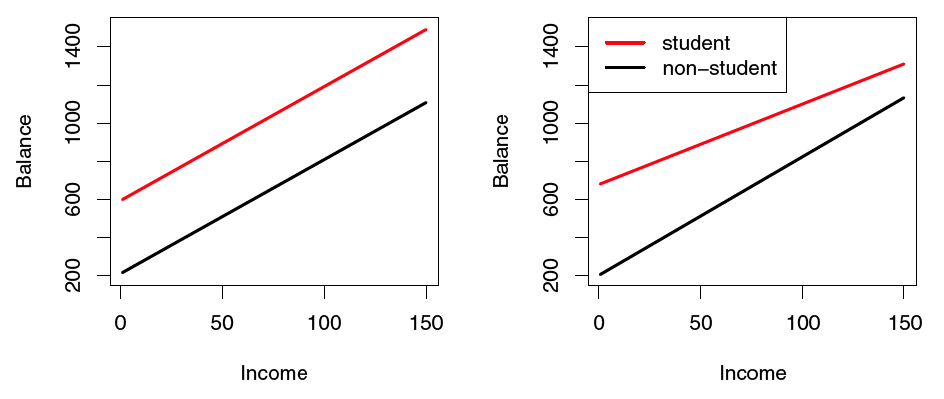
\includegraphics[width=0.9\textwidth]{images/islr/fig_3_7.png}
	\caption{Graficamos al modelo dado por la Ecuaci\'on \ref{eq:islr_3-34} a la izquierda, mientras que a la derecha graficamos el modelo dado por la Ecuaci\'on \ref{eq:islr_3-35}. Notamos que el t\'ermino de interacci\'on implica que cambios en el \vari{Income} est\'an asociados a incrementos m\'as peque\~nos en el \vari{Balance} para los estudiantes. Podemos encontrar los par\'ametros de las l\'ineas usando \texttt{est.params}.
	}
	\label{fig:islr_3-7}
\end{figure}
\end{frame}

\begin{frame}\frametitle{Relaciones No Lineales}
	\begin{itemize}
		\item Podemos usar una \defi{regresi\'on polinomial} para encontrar ajustes no lineales a los datos.
		\item Para los datos de \vari{Auto}, si graficamos \vari{horsepower} vs. \vari{mpg}, la figura nos sugiere una relaci\'on cuadr\'atica.
		\item Por ende, el modelo sugerido es:
		
		\begin{equation}\label{eq:islr_3-36}
		\vari{mpg} = \beta_0 + \beta_1 \times \vari{horsepower} + \beta_2 \times \vari{horsepower}^2 + \epsilon
		\end{equation}
		\item Podemos realizar la regresi\'on lineal agregando una columna a nuestros datos: \texttt{df["horsepower2"] = df.horsepower**2} y utilizando la ecuaci\'on \texttt{"mpg \textasciitilde  horsepower + horsepower2"}.
	\end{itemize}
\end{frame}

\begin{frame}\frametitle{\vari{mpg} vs.  \vari{horsepower} para los datos de \vari{Auto}}
\begin{figure}
	\centering
	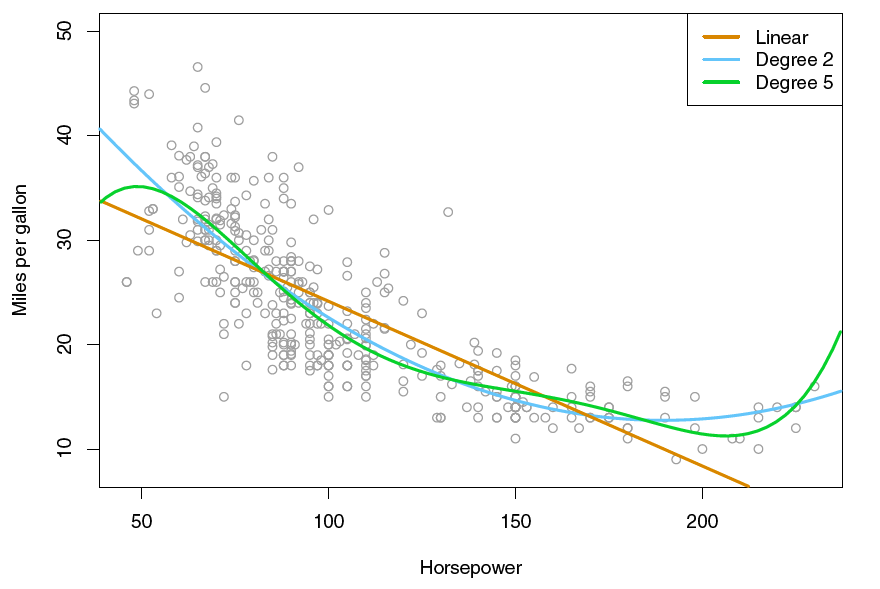
\includegraphics[width=0.65\textwidth]{images/islr/fig_3_8.png}
	\caption{La l\'inea \textcolor{orange}{naranja} es la recta de regresi\'on; la l\'inea \textcolor{Cerulean}{azul} es la curva de regresi\'on cuando el modelo incluye a $\vari{horsepower}^2$; la l\'inea \textcolor{green}{verde} es la curva de regresi\'on cuando el modelo incluye hasta la quinta potencia de \vari{horsepower}. N\'otese que $R^2=0.606$ para la regresi\'on lineal, $R^2=0.688$ para la cuadr\'atica y $R^2=0.697$ para la de grado 5.
	}
	\label{fig:islr_3-8}
\end{figure}
\end{frame}


\begin{frame}\frametitle{Posibles Problemas}
	\begin{itemize}
		\item Los problemas m\'as comunes a encontrar al realizar un  ajuste de regresi\'on lineal son:
		\begin{itemize}
			\item[1.] No linealidad de los datos
			\item[2.] Correlaci\'on de los t\'erminos de error
			\item[3.] Varianza no constante de los t\'erminos de error
			\item[4.] Valores at\'ipicos
			\item[5.] Puntos de alto apalancamiento
			\item[6.] Colinealidad
		\end{itemize}
	\item Tanto un arte como una ciencia.
	\end{itemize}
\end{frame}

\begin{frame}\frametitle{1. No linealidad de los datos}
	\begin{itemize}
		\item Si la relaci\'on de los datos es lejos de ser lineal, es posible que nuestras conclusiones pasadas sean falsas.
		\item Es \'util realizar \defi{gr\'aficos de residuos}, i.e., graficar $e_i=y_i-\hat y_i$ versus el predictor $x_i$.
		\item Para la regresi\'on lineal m\'ultliple, graficamos a $e_i$ vs. $\hat y_i$.
		\item Idealmente no debe de haber un patr\'on.
		\begin{itemize}
			\item De haberlo, se deben de realizar transformaciones no lineales a los datos. 
			\item Algunos comunes son $\log X$, $\sqrt{X}$, $X^2$, etc.
		\end{itemize}
		
	\end{itemize}
\end{frame}

\begin{frame}\frametitle{Gr\'afico de residuos para los datos de \vari{Auto}}
\begin{figure}
	\centering
	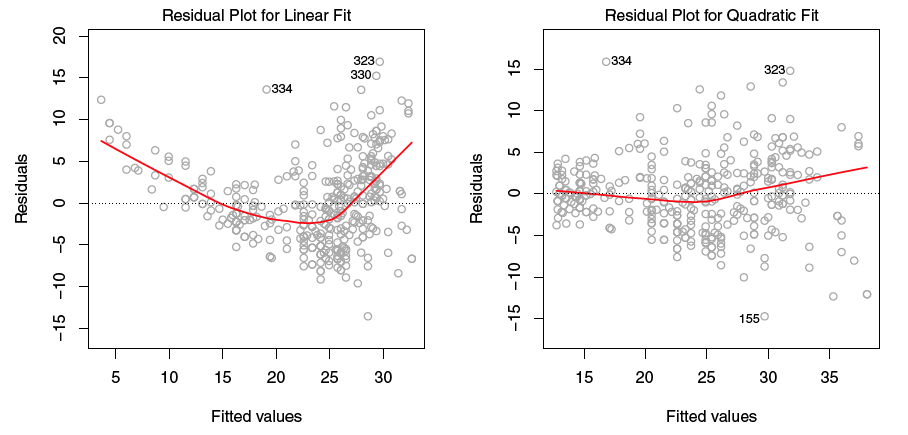
\includegraphics[width=0.9\textwidth]{images/islr/fig_3_9.png}
	\caption{Gr\'aficos de los residuos vs. los valores predichos del modelo ajustado a los datos de \vari{Auto}. La l\'inea roja est\'a ajustada a los residuos para ayudar a visualizar patrones. A la izquierda tenemos el modelo $\vari{mpg}\sim \vari{horsepower}$ y a la derecha el modelo $\vari{mpg}\sim\vari{horsepower}+ \vari{horsepower}^2$. Vemos que en la derecha no hay un patr\'on visible como en  la izquierda.
	}
	\label{fig:islr_3-9}
\end{figure}
\end{frame}

\begin{frame}[fragile]\frametitle{\href{https://github.com/JWarmenhoven/ISLR-python/blob/master/Notebooks/Chapter\%203.ipynb}{C\'odigo para gr\'afico de residuos (modelo lineal)}}
\begin{semiverbatim}
	\footnotesize{\textcolor{deepblue}{import} pandas \textcolor{deepblue}{as} pd
	\textcolor{deepblue}{import} seaborn \textcolor{deepblue}{as} sns
	\textcolor{deepblue}{from} sklearn.linear\_model \textcolor{deepblue}{import} skl\_lm
	
	auto = \href{https://pandas.pydata.org/pandas-docs/stable/generated/pandas.read_csv.html}{pd.read\_csv}("Auto.csv", index\_col=0)
	X=auto["horsepower"].values.reshape(-1,1)
	y= auto["mpg"]
	
	regr = skl\_lm.LinearRegression()
	
	model = regr.fit(X, y)
	
	auto["pred"] = model.predict(X)
	auto["resid"] = auto["mpg"]-auto["pred"]
	
	sns.regplot(auto["pred"], auto["resid"],  lowess=True, 
	            line\_kws=\{"color":"r", "lw":1\}, 
	            scatter\_kws=\{"facecolors":"None",
	                         "edgecolors":"k",
	                         "alpha":0.5\})}
	
	
\end{semiverbatim}
\end{frame}

\begin{frame}\frametitle{2. Correlaci\'on de los t\'erminos de error}
	\begin{itemize}
		\item Hemos asumido que los errores $\epsilon_1,\dots,\epsilon_n$ no est\'an correlacionados $\Rightarrow$ el signo de $\epsilon_i$ no nos dice nada del signo del $\epsilon_{i+1}$.
		\item Si est\'an correlacionados, entonces los errores est\'andar estimados van a subestimar los verdaderos errores est\'andar.
		\item Ocurre frecuentemente para las \defi{series temporales de datos}, en donde residuos adyacentes tienden  a tener los mismos valores (\defi{tracking}).
		\item Puede ocurrir tambi\'en fuera de las series temporales de datos.
		\begin{itemize}
			\item Por ejemplo, determinar la altura de un individuo en funci\'on de su peso. 
			\item Los errores tendr\'an una correlaci\'on si dos individuos son familiares, llevan la misma dieta, han sido expuestos a los mismos factores externos, etc.
		\end{itemize}
	\end{itemize}
\end{frame}

\begin{frame}\frametitle{Gr\'afico de residuos con distintos grados de correlaci\'on}
\begin{figure}
	\centering
	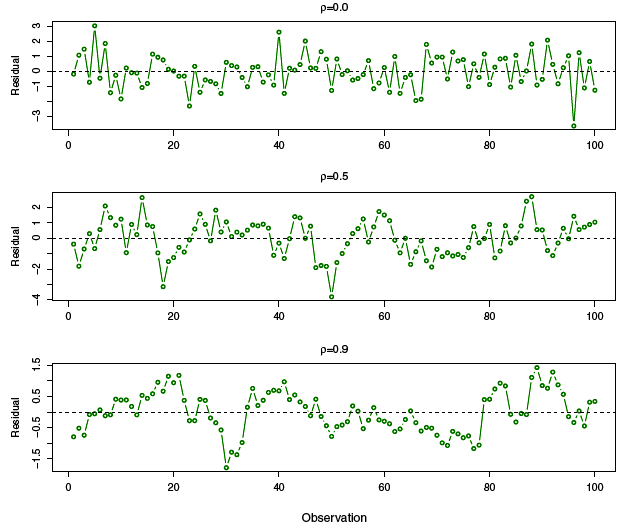
\includegraphics[width=0.5\textwidth]{images/islr/fig_3_10.png}
	\caption{Gr\'aficos de los residuos vs. valor observado para una serie temporal de datos simulada. Vemos el resultado para distintos grados de correlaci\'on, indicados por $\rho$. Mientras m\'as alto el valor de $\rho$, m\'as cercanos ser\'an los valores de los residuos adyacentes.
	}
	\label{fig:islr_3-10}
\end{figure}
\end{frame}

\begin{frame}\frametitle{3. Varianza no constante de los t\'erminos de error}
	\begin{itemize}
		\item Hemos asumido que $\mathbb{V}(\epsilon_i)=\sigma^2, \forall i$, pero esto puede no cumplirse.
		\item Podemos reconocer \'este efecto de \defi{heterocedasticidad} al observar que los residuos tienen forma de \textbf{embudo}.
		\item Una soluci\'on es transformar a $Y$ usando funciones c\'oncavas, como por ejemplo $\log Y$ o $\sqrt{Y}$.
	\end{itemize}
\end{frame}

\begin{frame}\frametitle{Heterocedasticidad}
\begin{figure}
	\centering
	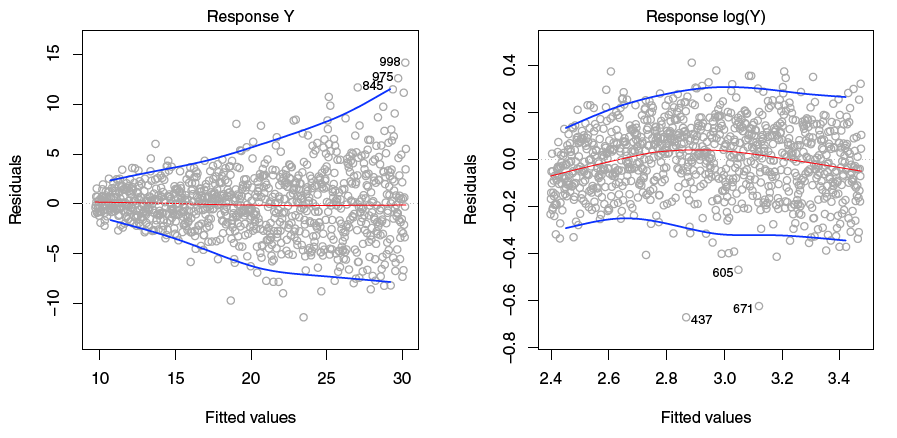
\includegraphics[width=0.85\textwidth]{images/islr/fig_3_11.png}
	\caption{Gr\'aficos de residuos para datos generados. La l\'inea \textcolor{red}{roja} es un ajuste suave de los residuos para visualizar m\'as f\'acilmente la tendencia. Las l\'ineas \textcolor{blue}{azules} nos muestran los cuantiles externos. A la izquierda, vemos la forma de embudo que caracteriza a la heterocedasticidad. A la derecha, hemos reealizado una transformaci\'on logar\'itmica a la respuesta, por lo que ya no hay evidencia de heterocedasticidad.
	}
	\label{fig:islr_3-11}
\end{figure}
\end{frame}

\begin{frame}\frametitle{4. Valores at\'ipicos}
	\begin{itemize}
		\item Un \defi{valor at\'ipico (outlier)} es un dato para el cual $y_i$ est\'a lejano al valor predicho por el modelo.
		\item No tienen mucho efecto en los coeficientes de la regresi\'on lineal, mas s\'i en el valor del $R^2$ y RSE, usados para calcular CI y valores p.
		\item Es dif\'icil determinar qu\'e tan grande debe de ser el residual para determinar si un valor es at\'ipico.
		\item Usualmente se realizan \defi{residuos estudentizados} y, de ser mayores a 3 o menores a -3, se clasifican como \textit{posibles} valores at\'ipicos.
		\item \textbf{Soluci\'on:} removerlos, aunque pueden indicar un la falta de un predictor, o bien una deficiencia del modelo.
	\end{itemize}
\end{frame}

\begin{frame}\frametitle{Valor at\'ipico}
\begin{figure}
	\centering
	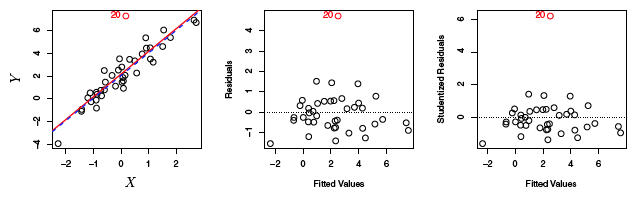
\includegraphics[width=0.8\textwidth]{images/islr/fig_3_12.png}
	\caption{A la izquierda vemos la recta de regresi\'on con todos los datos en \textcolor{red}{rojo} y la recta de regresi\'on sin el valor at\'ipico en \textcolor{blue}{azul}. Tendremos que $R^2=0.805$ y $\text{RSE}=1.09$ para a primera, $R^2=0.892$ y $\text{RSE}=0.77$ para la segunda. Al centro el gr\'afico de residuos nos muestra m\'as claramente al valor at\'ipico, pero quiz\'a hayan otros m\'as. A la derecha, graficando los residuos estudentizados nos permite observar que todos los valores, menos el at\'ipico, tienen un residuo estudentizado menor a 2 en valor absoluto.
	}
	\label{fig:islr_3-12}
\end{figure}
\end{frame}

\begin{frame}\frametitle{5. Puntos de alto apalancamiento}
	\begin{itemize}
		\item Las observaciones con \defi{alto apalancamiento} tienen  un valor inusual para $x_i$.
		\item Calculamos el \defi{estad\'istico de apalancamiento}:
		\begin{equation}\label{eq:islr_3-37}
		h_i = \frac{1}{n}+\frac{(x_i-\bar{x})^2}{\sum_{i'=1}^{n}(x_{i'}-\bar{x})^2}
		\end{equation}
		\begin{itemize}
			\item Es la $i-$\'esima entrada en la diagonal de $\matr{H}=\matr{X}(\matr{X}^{\top }\matr{X})^{-1}\matr{X}^{\top }$
		\end{itemize}
		\item Mientras mayor sea, nos indicar\'a que una observaci\'on tiene alto apalancamiento.
		\item $h_i$ aumenta conforme m\'as se aleje la observaci\'on del promedio, por lo que $h_i\in [1/n,1]$.
		\item El apalancamiento promedio para todas las observaciones es de $(p+1)/n$, con lo que podemos comparar para ver si una observaci\'on tiene alto apalancamiento.
	\end{itemize}
\end{frame}

\begin{frame}\frametitle{Apalancamiento}
\begin{figure}
	\centering
	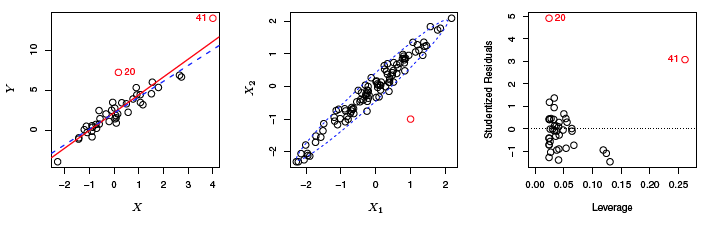
\includegraphics[width=0.8\textwidth]{images/islr/fig_3_13.png}
	\caption{La observaci\'on \textbf{41} que tiene alto apalancamiento, mientras que la \textbf{20} no. A la izquierda vemos la recta de regresi\'on con todos los datos en \textcolor{red}{rojo} y la recta de regresi\'on (sin incluir a la observaci\'on \textbf{41})  en \textcolor{blue}{azul}. Vemos que dicho valor tiene mayor efecto sobre la recta que la observaci\'on \textbf{20}. Al centro, vemos para $p=2$ que la observaci\'on en \textcolor{red}{rojo} no tiene un valor inusual para $X_1$ o $X_2$, pero yace fuera del grupo de datos. A ls derecha, graficamos al apalancamiento vs. residuos estudientizados. Notamos entoncees que la observaci\'on \textbf{20} es un valor at\'ipico con bajo apalancamiento, mientras que la observaci\'on \textbf{41} es un valor at\'ipico con alto apalancamiento.
	}
	\label{fig:islr_3-13}
\end{figure}
\end{frame}

\begin{frame}\frametitle{6. Colinealidad (1)}
	\begin{itemize}
		\item \defi{Colinealidad} se refiere a la situaci\'on en donde dos o m\'as predictores est\'an relacionados unos a otros.
		\item E.g., para los datos de \vari{Credit}, \vari{Limit} y \vari{Age} se dicen que son \defi{colineales}.
		\item Colinealidad hace que crezcan los $\text{SE}(\hat\beta_j)$, lo que hace que el estad\'istico t se reduzca.
		\item Como resultado, podr\'iamos no poder rechazar a $H_0:\beta_j=0$.
		\item La forma m\'as sencilla de detectar colinealidad es observando los valores de la matriz de correlaci\'on $\matr{M}$.
	\end{itemize}
\end{frame}

\begin{frame}\frametitle{Colinealidad}
\begin{figure}
	\centering
	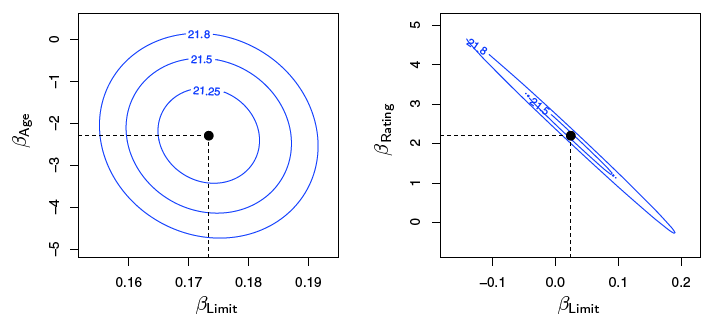
\includegraphics[width=0.8\textwidth]{images/islr/fig_3_15.png}
	\caption{Gr\'aficas de contorno para los valores de RSS en funci\'on de los par\'ametros usando a los datos de \vari{Credit}. El punto negro indica el valor \'optimo de $\beta$. A la izquierda, tenemos los contornos de RSS para el modelo $\vari{Balance}\sim\vari{Age}+\vari{Limit}$
	, mientras que a la derecha tenemos el modelo $\vari{Balance}\sim\vari{Rating}+\vari{Limit}$. Debido a la colinealidad, no es tan claro cu\'al es el valor de $(\beta_{\text{\vari{Limit}}}, \beta_{\text{\vari{Rating}}})$ que minimiza al RSS.
	} 
	\label{fig:islr_3-15}
\end{figure}
\end{frame}

\begin{frame}\frametitle{6. Colinealidad (2)}
\begin{itemize}
	\item Es posible que exista colinealidad entre tres o m\'as variables, aunque no exista colinealidad entre los pares de variables.
	\item Llamamos a esto \defi{multicolinealidad} y debemos de calculalo usando el \defi{factor de inflaci\'on de la varianza (VIF)}:
	\begin{equation}\label{eq:islr_vif}
		\text{VIF}(\hat\beta_j)=\frac{1}{1-R_{X_j |X_{-j}}^{2}}
	\end{equation}
	donde $R_{X_j |X_{-j}}^{2}$ es el $R^2$ de una regresi\'on de $X_j$ sobre todos los otros predictores.
	\begin{itemize}
		\item Su valor m\'inimo es 1.
		\item Si es mayor a 5 o 10, nos indica que hay un problema de colinealidad.
	\end{itemize}
	\item \textbf{Soluci\'on:} botar una de las variables, o bien combinarlas para formar otra variable.
\end{itemize}
\end{frame}

\begin{frame}[fragile]\frametitle{C\'odigo para VIF}
\begin{semiverbatim}
	\scriptsize{\textcolor{deepblue}{import} pandas \textcolor{deepblue}{as} pd
	\textcolor{deepblue}{import} numpy \textcolor{deepblue}{as} np
	\href{https://www.statsmodels.org/dev/generated/statsmodels.stats.outliers_influence.variance_inflation_factor.html}{\textcolor{deepblue}{from} statsmodels.stats.outliers\_influence \textcolor{deepblue}{import} variance\_inflation\_factor}
	\href{https://patsy.readthedocs.io/en/latest/API-reference.html}{\textcolor{deepblue}{from} patsy \textcolor{deepblue}{import} dmatrices}
	
	credit = pd.read\_csv("Crefit.csv", index\_col=0).\href{https://pandas.pydata.org/pandas-docs/stable/generated/pandas.DataFrame.dropna.html}{dropna()}.\href{https://github.com/pandas-dev/pandas/blob/870b6a6d6415c76d051b287adcb180ac3020b6e8/pandas/core/generic.py#L3538}{\_get\_numeric\_data()}

	y, X = dmatrices("Balance ~ Age+Rating+Limit", credit, return\_type="dataframe")
	
	cols=X.shape[1]
	
	vif = pd.DataFrame()
	
	vif["features"] = X.columns
	vif["VIF Factor"] =[variance\_inflation\_factor(X.values, i) for i in range(cols)]
	vif.index = np.arange(1, len(vif)+1)
	
	>>> vif.round(2)
	    Features  VIF Factor
	1  Intercept       23.80
	2        Age        1.01
	3     Rating      160.67
	4      Limit      160.59
	}
	
\end{semiverbatim}
\end{frame}

\end{document}